% Use only LaTeX2e, calling the article.cls class and 12-point type.

\documentclass[12pt]{article}

% Users of the {thebibliography} environment or BibTeX should use the
% scicite.sty package, downloadable from *Science* at
% www.sciencemag.org/about/authors/prep/TeX_help/ .
% This package should properly format in-text
% reference calls and reference-list numbers.

\usepackage{scicite}
\usepackage{graphicx}

% Use times if you have the font installed; otherwise, comment out the
% following line.

\usepackage{times}

% The preamble here sets up a lot of new/revised commands and
% environments.  It's annoying, but please do *not* try to strip these
% out into a separate .sty file (which could lead to the loss of some
% information when we convert the file to other formats).  Instead, keep
% them in the preamble of your main LaTeX source file.


% The following parameters seem to provide a reasonable page setup.

\topmargin 0.0cm
\oddsidemargin 0.2cm
\textwidth 16cm 
\textheight 21cm
\footskip 1.0cm


%The next command sets up an environment for the abstract to your paper.

\newenvironment{sciabstract}{%
\begin{quote} \bf}
{\end{quote}}


% If your reference list includes text notes as well as references,
% include the following line; otherwise, comment it out.

%\renewcommand\refname{References and Notes}


% Include your paper's title here

\title{Micromouse: Designing an Educational Racing-Robot from Scratch \\Report} 



% Place the author information here.  Please hand-code the contact
% information and notecalls; do *not* use \footnote commands.  Let the
% author contact information appear immediately below the author names
% as shown.  We would also prefer that you don't change the type-size
% settings shown here.

% I think we should organize our names alphabetically
\author
{Natalia Poliakova,$^{1}$ Autor 2,$^{2}$, Autor 3$^{3}$, Autor 4, $^{4}$ Autor 5, $^{5}$ Autor 6 $^{6}$\\
\\
\normalsize{$^{1}$Department of Informatics, Technical University of Munich}\\
\normalsize{An Unknown Address, Wherever, ST 00000, USA}\\
\normalsize{$^{2}$Another Unknown Address, Palookaville, ST 99999, USA}\\
\\
}

% Include the date command, but leave its argument blank.

\date{}



%%%%%%%%%%%%%%%%% END OF PREAMBLE %%%%%%%%%%%%%%%%



\begin{document} 

% Double-space the manuscript.

\baselineskip24pt

% Make the title.

\maketitle 

% Place your abstract within the special {sciabstract} environment.

\begin{sciabstract}
    Our abstract - short overview of the whole report contents? Probably should be left untouched till we finish with the main report body.
\end{sciabstract}

\newpage

\tableofcontents



% In setting up this template for *Science* papers, we've used both
% the \section* command and the \paragraph* command for topical
% divisions.  Which you use will of course depend on the type of paper
% you're writing.  Review Articles tend to have displayed headings, for
% which \section* is more appropriate; Research Articles, when they have
% formal topical divisions at all, tend to signal them with bold text
% that runs into the paragraph, for which \paragraph* is the right
% choice.  Either way, use the asterisk (*) modifier, as shown, to
% suppress numbering.

\newpage


\section{Introduction}

\subsection{Micromouse competition}

According to the general description of the micromouse competition, "in this contest the contestant, or team of contestants, must design and build an autonomous robotic ”mouse” capable of traversing a maze of standard dimensions from a specified corner to its center in the shortest time." \cite{MicromouseRules}.\\
General example of a competition setup can be seen on the Fig.~\ref{fig:micromouse}. 
\begin{figure}[htb]
    \centering
    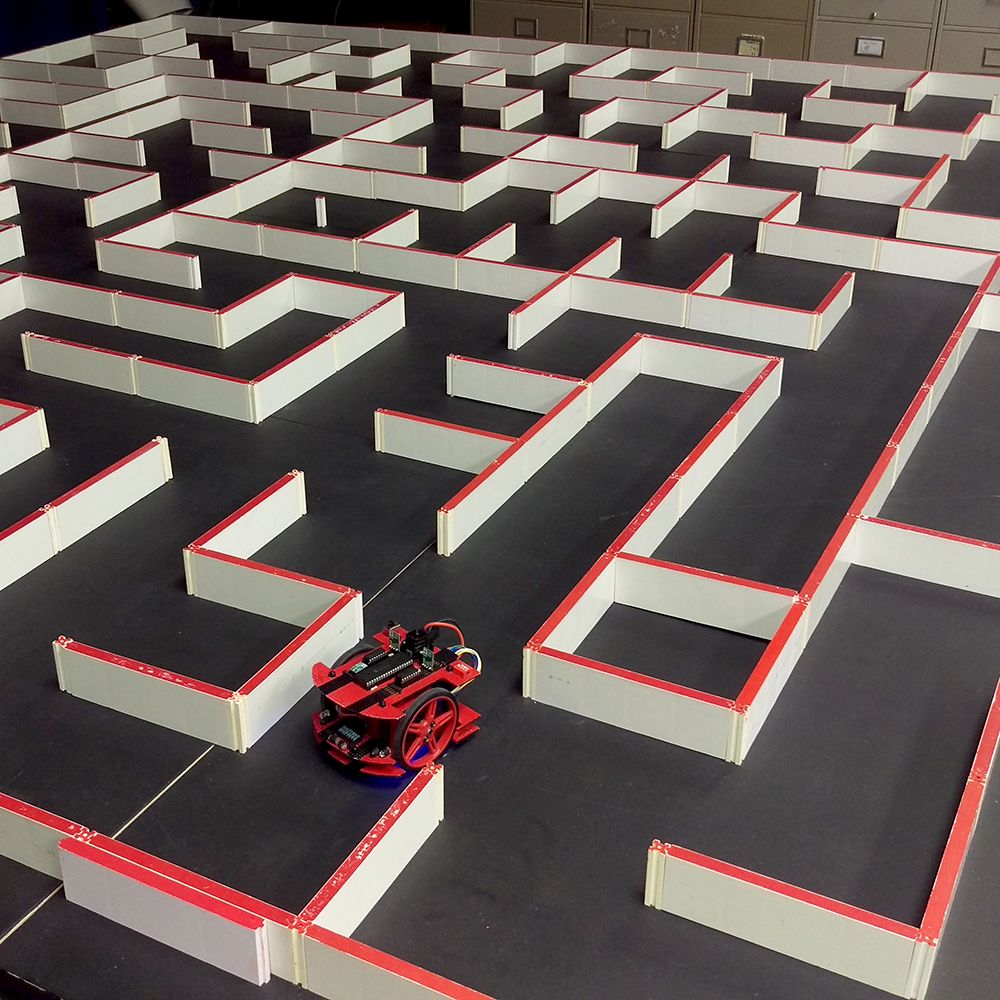
\includegraphics[width=0.6\textwidth]{figures/micromouse-maze.jpg}
    \caption{Micromouse competition photo: labyrinth and robot example \cite{MicromousePhotoLink}}
    \label{fig:micromouse}
\end{figure}

\subsection{Aims and Objectives}

    Short summary of the general competition rules is as following \cite{MicromouseRules}:

\begin{itemize}
    \item Self-Containment: A Micromouse shall be self-contained (no remote controls).
    \item Method of Movement: A Micromouse shall not jump over, fly over, climb, scratch,cut, burn, mark, damage, or destroy the walls of the maze.
    \item Maze Dimensions: The maze is composed of 18cm x 18cm unit squares arranged as 16 x 16 units. The walls of the units of the maze are 5 cm high and 1.2 cm thick 
    \item Multiple Paths: Multiple paths to the destination square are allowed and are to be expected. The destination square will be positioned so that a wall-hugging mouse will NOT be able to find it.
\end{itemize}
    
 In the case of our project, the aforementioned rules were used in a slightly modified way. The labyrinth is reduced in size to 8x8 units in order to fit better to the project conditions. The micromouse competition consists of 2 runs: in the first run, the robot is going through the maze and, according to arbitrary chosen algorithm, constructs the maze map; in the second run the mouse should reach the center of the maze (found in the first run) as quickly as possible, according to the composed map of the labyrinth. \\
 The main goal of the project was set to:  "get as close to the realization of the procedure described above as possible".
 The ways and approaches that were chosen to reach this goal are named and described properly in the next section.
 
 \subsection{Tools}
 
The list of tools used throughout the whole length of the project:
\begin{itemize}
    \item Microchip MPLABX - an IDE, used to set-up, configure and program a microcontroller. Used together with XC16 compiler from Microchip.
    \item MathWorks MATLAB \textcolor{red}{(did any of us except for Alex actually use it?)}
    \item Autodesk Eagle - PCB design software, used to create schematic diagrams, organize the component placement and route the PCB.
    \item Autodesk Fusion 360 -  CAD/CAM design software, used to build in 3D all parts of the casing for the robot.
\end{itemize}



\section{Conceptual design and justification of the design}

In order to set the right design goals and milestones during the semester, adequately estimate the workload and organize the working process in the most effective way, we needed to: analyze the initial design conditions and restrictions, roughly formulate the implementation blocks along with respective skill-sets of all project members and - after that - write down the most suitable working program. Both steps are described in detail below.

\subsection{Initial design conditions} \label{chap:design_cond}
The main question to answer was to grasp and implement using the knowledge we had acquired plus the logic behind the "how do we build a robot that should drive in the labyrinth and be able to make intelligent decisions (turns) based on the observations (made by sensors)"?

\noindent 
There are some predefined conditions and tools that we used as a starting point in answering this question: 

\begin{itemize}
    \item Geometric constraints\\ 
    As was mentioned in the previous section, the geometric parameters of the maze in our case were as following: 8x8 identical squares with a side of 16cm. Therefore, our "mouse" was logically required to be smaller than 16cm in width and length, ideally the size that would allow it to move freely while performing any type of movement within the maze (therefore leaving at least 2-3 centimeters of distance to the surrounding walls)
    \item Power supply\\
    According to the unified formal requirements of the Micromouse competition, the robot should be autonomous, which infers carrying it's own power supply in form of a standard 9V battery.
    \item Sensing the environment\\
    The initial condition in regards to sensing simply states that the robot should be able to perceive the environment and make informed decisions about the next movement (moving straight or turning in one of the directions - the turn angle was set to be fixed at 90 degrees in order to simplify the design) based on the analysis of the information received from the sensors. The sensor type that is the most efficient for the cause - simple infrared proximity sensor. We had an option to either order the desired amount of sensors or to build them ourselves.
    \item Motors\\
    In order for the "mouse" to move, we were provided with predefined 2619-SR-IE2-16 motors and sets of wheels of different diameter.
    \item Microcontroller\\
    Initially, for the educational purposes and in order to gain some knowledge in configuring and setting up the microcontroller to control the needed peripherals, a pair of dsPIC30F4011 microcontrollers was provided. Appropriate for the goal task microcontroller was decided to be chosen later. Overall, it had to have all required pins and interfaces, such as:\\
    - PWM outputs for the motor control\\
    - analog inputs to receive data from sensors\\
    - enough extra pins to connect peripherals (such as LEDs)\\
    - flexible and convenient pin mapping in order to satisfy the geometric constraints
    \item PCB\\
    The printed circuit board for the robot was to be designed independently, according to all the aforementioned conditions.
    \item Casing\\
    In order for all of the components (such as the board, the motors and the battery) to hold together in one single "mouse" unit, it was set that a custom casing must be designed and printed.
\end{itemize}

Based on those conditions and also tools and devices provided, we came up with the implementation plan, which can be seen in detail in the next part.

\subsection{Work program and Gantt chart}
In the below Fig. \ref{fig:gantt}, we describe our planned stages within a Gantt chart.

\begin{figure}[H]
    \centering
    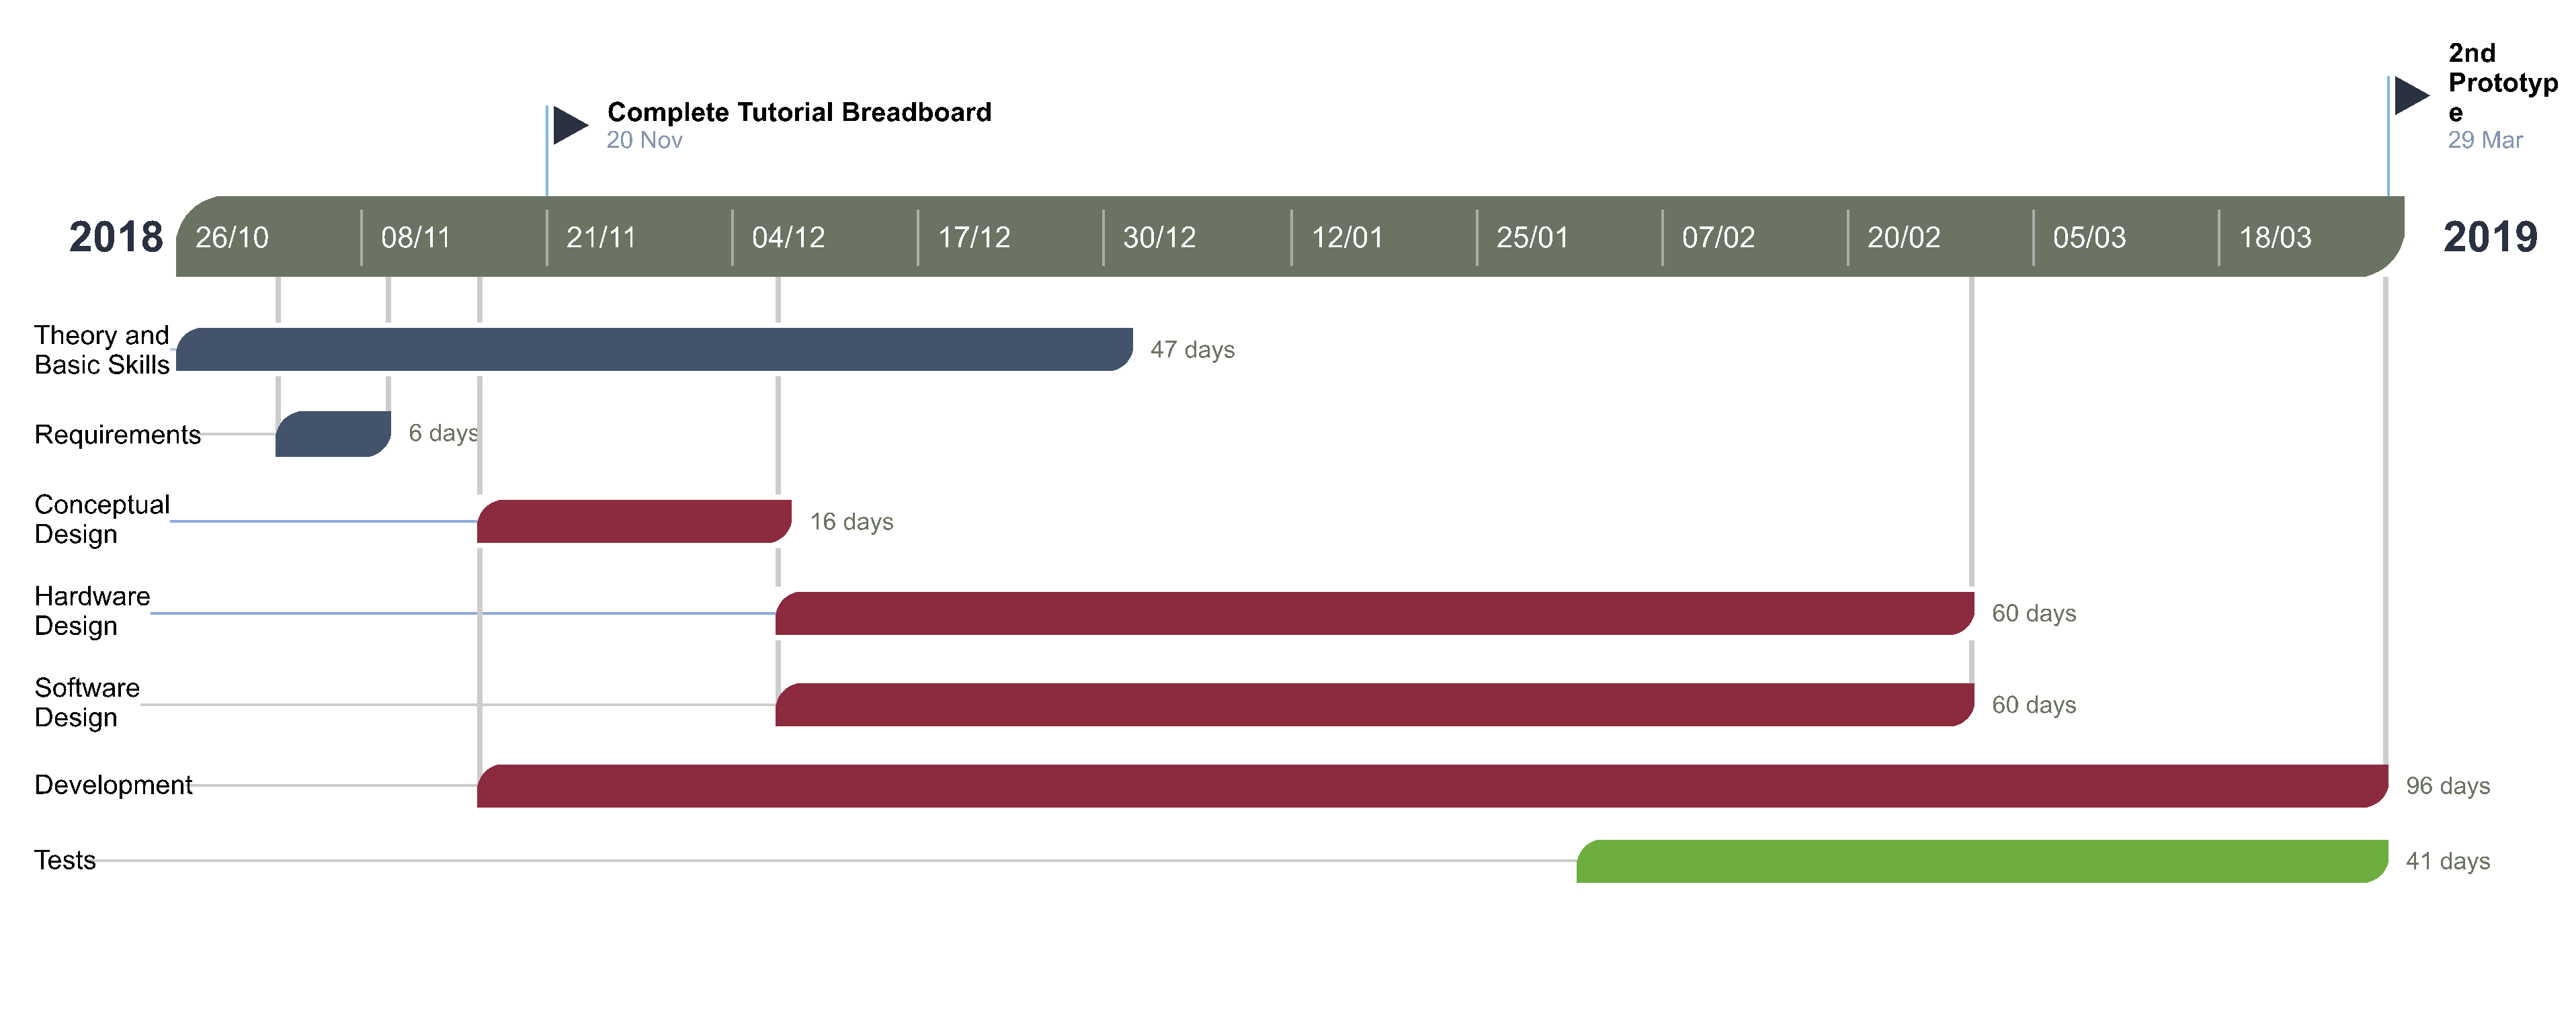
\includegraphics[width=1\textwidth]{figures/micromouse-gantt.png}
    \caption{Gantt chart of our progress}
    \label{fig:gantt}
\end{figure}

\noindent
In the first half of the semester we started off with a basic introduction to electrical engineering. By using the microcontroller dsPIC30F4012 we followed a practical course and learned to use the Microchip MPLABX environment in order to create and simulate the code for the software of the micromouse.

\noindent
The practial course was comprised of the following topics:
\begin{itemize}
    \item Digital I/O
    \item Interrupts
    \item PWM
    \item UART
    \item Quadrature Encoders
    \item Analogue Inputs
\end{itemize}

\noindent
During the practial course we applied our learnings onto a breadboard. Which can be seen in Fig. \ref{fig:breadboard}. By doing this we got an idea of what kind of electronic parts we will need to get accustomed with for the creation of the final micromouse. Our acquired knowledge will be described in more detail in the next chapter.

\begin{figure}[H]
    \centering
    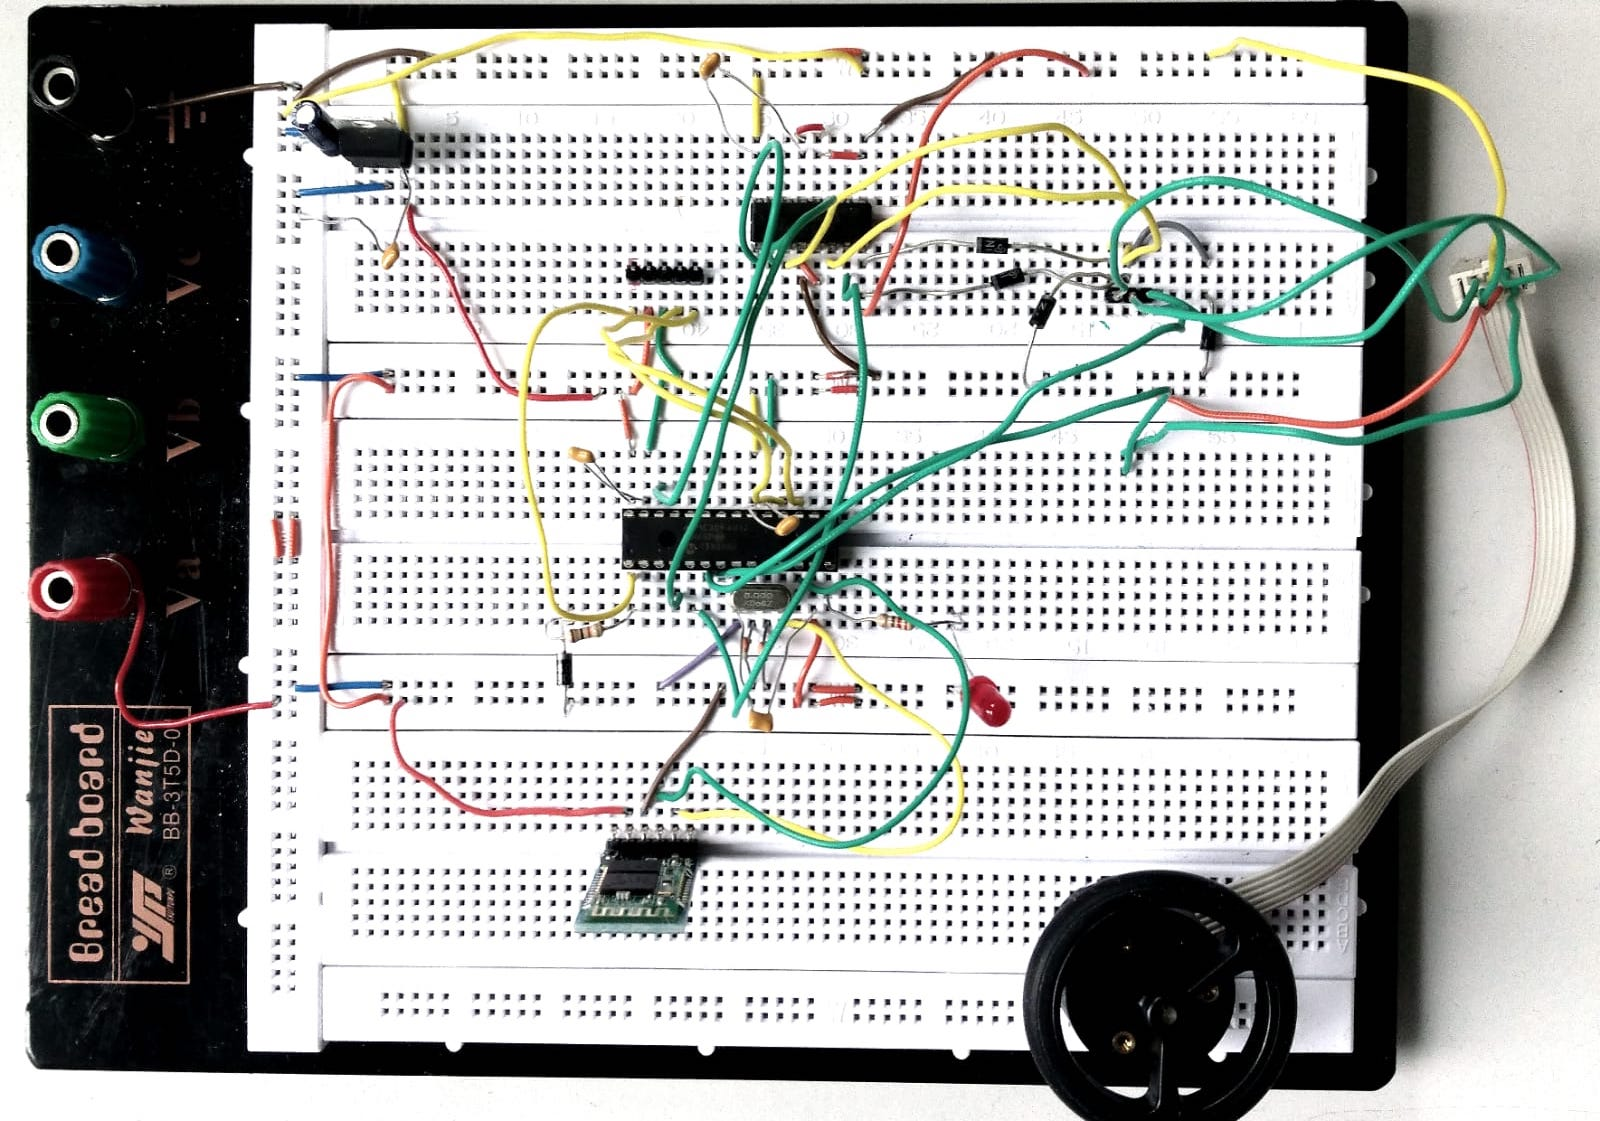
\includegraphics[width=0.6\textwidth]{figures/hardware/breadboard.jpeg}
    \caption{First completed breadboard}
    \label{fig:breadboard}
\end{figure}

\noindent
While going through the practical course, we fetched all the requirements we would need during the preparations of building the micromouse. All of them are described in the previous chapter \ref{chap:design_cond} \\

\noindent
The former idea of splitting us students into two separate groups was canceled because it took us too long to complete the basic introduction (as it was initially planned) plus the fact that we all were inexperienced in electrical engineering. Instead we formed two teams: One was responsible for the hardware the other one for the software design. This and other issues are mentioned in chapter \ref{chap:challenges}.\\
So after all requirements were known and the conceptual design phase was completed, we started with designing the hardware and software. Both are described in more detail in the chapters \ref{chap:hardware} and \ref{chap:software} respectively. \\
In order to construct a PCB with all the parts we need, we are using Autodesk Eagle. For writing the software we are using the MPLABX environment. \\

\noindent
The testing part concludes the overall development stage. But because testing is such a crucial element during a development, especially when designing hardware is a part of it, every step has to be done with caution. Hence, a failure of an electrical compound can easily lead to a broken part, which will result in unnecessary costs and time delays. The test results can be found in chapter \ref{chap:tests}. \\

\textcolor{red}{I would suggest to fit here the part with "design decisions based on the aforementioned conditions (justification)"
\textit{ This is where I'm a bit lost. We could include some "ideal" version of this chart here, but where exactly should we describe all the changes in planning and organization and why they had to be done at each stage of building the prototype and the final version of the mouse?  Should it be described here? Or later in the "problems and challenges"?
Also I think maybe here we should talk about all the initial learning stage we had to go through in the first half of the praktikum (maybe devote a subsection for this here or later in the report)}}



\section{Hardware and software design}

Some introductory info

\subsection{Hardware design}

    \subsubsection{Board design}

    The complete description of our schematics design and board design and what we did and why
    Also including all calculations we've managed to collect throughout the whole course of said design.
    Pretty pictures and some tables with calculated values would be amazing.

    \subsubsection{Casing design}

    The whole journey on the casing design. Pictures of the final 3D model and printed model of course, some calculations and data on the sizes and maybe geometrical values 
    
\subsection{Software design}

    The description of our modular architecture, the work principles of the separate modules and basically "how we control the peripherals" such as motors, leds, timers, etc. Logic comes a bit later in here.
    Also all info on DMA and pin remapping and our pretty mapping table are also welcomed here I think




\section{Controller Design and Approach}

Here goes the whole logic of the mouse movement control (how should it behave when is faced with the wall or on contrary - with the gap in the labyrinth). PID controller design and the logic behind it.




\section{Summary of tests}

Here goes everything practical we could possibly test - for example the speeding curve of the motor, the temperature conditions of the board (when we'll solder it - whether it is able to work without overheating and such) 
Of course, the PID working values (such as the error convergence rate)
Possible subsections:\\
    - casing tests \\
    - schematic tests \\
    - software logic tests \\





\section{Implementation challenges}
Some general words about our journey with the mouse.

\subsection{Summary of problems encountered}
Well, here go all the problems we faced coupled with our solutions for them. Potentially the longest part in the report. Can be split in parts similarly to the previous sections (talking about software, board and casing)

\subsection{Learning experience} %the name is terrible, please smb name it properly, I'm out of imagination

What we learned basically? What was especially hard to grasp, e.t.c.
We could somehow present it as the short submission from each of us (as well as the previous part) Here we could also put the story of the first half of the semester (at least in the summarized form) and what concepts and practices and stuff we learned from that.





\section{Conclusions}
Here - short summary of the achieved results, maybe some general words and praises for our final mouse version, just something positive to end the mouse story well.

\subsection{Expectations}
Slightly controversial part, we could omit it (I would like not to though) or rephrase it somehow. Basically - what did we expect from the course. Not sure if this part actually belongs here, but for now it works.
\subsection{Propositions}
Our suggestions to maybe somehow improve or better organize some parts of the praktikum or the task or whatever.




\newpage
\section*{Appendix}
some extra figures

\vspace{3cm}

\bibliography{scibib}

\bibliographystyle{Science}

\newpage

Some guidelines from the template
\vspace{5cm}
\begin{enumerate}
\item Please follow the style for references outlined at our author
  help site and embodied in recent issues of {\it Science}.  Each
  citation number should refer to a single reference; please do not
  concatenate several references under a single number.
\item Please cite your references and notes in text {\it only\/} using
  the standard \LaTeX\ \verb+\cite+ command, not another command
  driven by outside macros.
\item Please separate multiple citations within a single \verb+\cite+
  command using commas only; there should be {\it no space\/}
  between reference keynames.  That is, if you are citing two
  papers whose bibliography keys are \texttt{keyname1} and
  \texttt{keyname2}, the in-text cite should read
  \verb+\cite{keyname1,keyname2}+, {\it not\/}
  \verb+\cite{keyname1, keyname2}+.
\end{enumerate}

\noindent Failure to follow these guidelines could lead
to the omission of the references in an accepted paper when the source
file is translated to Word via HTML.

\section*{Handling Math, Tables, and Figures}

Following are a few things to keep in mind in coding equations,
tables, and figures for submission to {\it Science}.

\paragraph*{In-line math.}  The utility that we use for converting
from \LaTeX\ to HTML handles in-line math relatively well.  It is best
to avoid using built-up fractions in in-line equations, and going for
the more boring ``slash'' presentation whenever possible --- that is,
for \verb+$a/b$+ (which comes out as $a/b$) rather than
\verb+$\frac{a}{b}$+ (which compiles as $\frac{a}{b}$).  Likewise,
HTML isn't tooled to handle certain overaccented special characters
in-line; for $\hat{\alpha}$ (coded \verb+$\hat{\alpha}$+), for
example, the HTML translation code will return [\^{}$(\alpha)$].
Don't drive yourself crazy --- but if it's possible to avoid such
constructs, please do so.  Please do not code arrays or matrices as
in-line math; display them instead.  And please keep your coding as
\TeX-y as possible --- avoid using specialized math macro packages
like \texttt{amstex.sty}.

\paragraph*{Displayed math.} Our HTML converter sets up \TeX\
displayed equations using nested HTML tables.  That works well for an
HTML presentation, but Word chokes when it comes across a nested
table in an HTML file.  We surmount that problem by simply cutting the
displayed equations out of the HTML before it's imported into Word,
and then replacing them in the Word document using either images or
equations generated by a Word equation editor.  Strictly speaking,
this procedure doesn't bear on how you should prepare your manuscript
--- although, for reasons best consigned to a note, we'd
prefer that you use native \TeX\ commands within displayed-math
environments, rather than \LaTeX\ sub-environments.

\paragraph*{Tables.}  The HTML converter that we use seems to handle
reasonably well simple tables generated using the \LaTeX\
\texttt{\{tabular\}} environment.  For very complicated tables, you
may want to consider generating them in a word processing program and
including them as a separate file.

\paragraph*{Figures.}  Figure callouts within the text should not be
in the form of \LaTeX\ references, but should simply be typed in ---
that is, \verb+(Fig. 1)+ rather than \verb+\ref{fig1}+.  For the
figures themselves, treatment can differ depending on whether the
manuscript is an initial submission or a final revision for acceptance
and publication.  For an initial submission and review copy, you can
use the \LaTeX\ \verb+{figure}+ environment and the
\verb+\includegraphics+ command to include your PostScript figures at
the end of the compiled PostScript file.  For the final revision,
however, the \verb+{figure}+ environment should {\it not\/} be used;
instead, the figure captions themselves should be typed in as regular
text at the end of the source file (an example is included here), and
the figures should be uploaded separately according to the Art
Department's instructions.


\section*{What to Send In}

What you should send to {\it Science\/} will depend on the stage your manuscript is in:

\begin{itemize}
\item {\bf Important:} If you're sending in the initial submission of
  your manuscript (that is, the copy for evaluation and peer review),
  please send in {\it only\/} a PostScript or PDF version of the
  compiled file (including figures).  Please do not send in the \TeX\ 
  source, \texttt{.sty}, \texttt{.bbl}, or other associated files with
  your initial submission.  (For more information, please see the
  instructions at our Web submission site,
  http://www.submit2science.org/ .)
\item When the time comes for you to send in your revised final
  manuscript (i.e., after peer review), we require that you include
  all source files and generated files in your upload.  Thus, if the
  name of your main source document is \texttt{ltxfile.tex}, you
  need to include:
\begin{itemize}
\item \texttt{ltxfile.tex}.
\item \texttt{ltxfile.aux}, the auxilliary file generated by the
  compilation.
\item A PostScript file (compiled using \texttt{dvips} or some other
  driver) of the \texttt{.dvi} file generated from
  \texttt{ltxfile.tex}, or a PDF file distilled from that
  PostScript.  You do not need to include the actual \texttt{.dvi}
  file in your upload.
\item From B{\small{IB}}\TeX\ users, your bibliography (\texttt{.bib})
  file, {\it and\/} the generated file \texttt{ltxfile.bbl} created
  when you run B{\small{IB}}\TeX.
\item Any additional \texttt{.sty} and \texttt{.bst} files called by
  the source code (though, for reasons noted earlier, we {\it
    strongly\/} discourage the use of such files beyond those
  mentioned in this document).
\end{itemize}
\end{itemize}

% Your references go at the end of the main text, and before the
% figures.  For this document we've used BibTeX, the .bib file
% scibib.bib, and the .bst file Science.bst.  The package scicite.sty
% was included to format the reference numbers according to *Science*
% style.


\bibliography{scibib}

\bibliographystyle{Science}



% Following is a new environment, {scilastnote}, that's defined in the
% preamble and that allows authors to add a reference at the end of the
% list that's not signaled in the text; such references are used in
% *Science* for acknowledgments of funding, help, etc.


% For your review copy (i.e., the file you initially send in for
% evaluation), you can use the {figure} environment and the
% \includegraphics command to stream your figures into the text, placing
% all figures at the end.  For the final, revised manuscript for
% acceptance and production, however, PostScript or other graphics
% should not be streamed into your compliled file.  Instead, set
% captions as simple paragraphs (with a \noindent tag), setting them
% off from the rest of the text with a \clearpage as shown  below, and
% submit figures as separate files according to the Art Department's
% instructions.


\end{document}




















